\documentclass[preprint,12pt]{elsarticle}

\usepackage{amsmath,amssymb,mathtools}
\usepackage{booktabs}
\usepackage{multirow}
\usepackage{graphicx}
\usepackage{xcolor}
\usepackage{microtype}
\usepackage{enumitem}
\usepackage{siunitx}
\usepackage{xurl}
\usepackage[section]{placeins}
\renewcommand{\topfraction}{0.9}
\renewcommand{\textfraction}{0.08}
\usepackage[hidelinks]{hyperref}
\pdfstringdefDisableCommands{\def\corref#1{}}

\journal{Knowledge-Based Systems}
\graphicspath{{../figures/out/}}
\definecolor{stablegreen}{HTML}{007C78}
\definecolor{stableorange}{HTML}{D97706}
\newcommand{\StableKG}{\textsc{StableKG}}
\newcommand{\ie}{i.e.,\ }
\newcommand{\eg}{e.g.,\ }

\makeatletter
\setlength{\@fptop}{0pt}
\setlength{\@fpsep}{16pt}
\setlength{\@fpbot}{0pt plus 1fil}
\makeatother
\begin{document}

\begin{frontmatter}

\title{Stability certificates for selective reasoning over evolving knowledge graphs}

\author[inst1]{Yanbo Bian\corref{cor1}}
\ead{24722081@bjtu.edu.cn}
\cortext[cor1]{Corresponding author}
\address[inst1]{Computer Science and Technology, Beijing Jiaotong University Weihai International College, Weihai, China}

\begin{abstract}
Evolving knowledge graphs require a decision beyond ranking missing facts: which predictions remain usable when their supporting evidence changes? We introduce \StableKG{}, a selective reasoning protocol that couples calibrated belief with explicit evidence-deletion diagnostics. Under an additive temporal evidence model, a window-count certificate gives the smallest number of supporting windows whose deletion erases a positive winner margin. The associated removal cost and temporal diversity describe how support is distributed; a validation-trained selector combines them with the normalized evidence margin to decide when to accept or abstain. Across ICEWS14 and ICEWS05-15, the selector reduces area under the risk--coverage curve from 0.5872 to 0.5494 and from 0.5011 to 0.4669, respectively. Improvements persist with a learned temporal backbone and when events are revealed chronologically. Matched feature controls identify the normalized margin as a major contributor to selective accuracy, while direct evidence edits establish the diagnostic value of temporal support structure. A separate controlled dependency-graph experiment reduces recomputation work by 71.6\% and propagation time by 47.7\%, preserving exact agreement with full recomputation. By connecting prediction, evidence sensitivity and selective acceptance, \StableKG{} provides an inspectable decision protocol for reasoning over changing knowledge.
\end{abstract}

\begin{keyword}
temporal knowledge graph \sep selective prediction \sep uncertainty calibration \sep evidence stability \sep incremental reasoning \sep abstention
\end{keyword}

\end{frontmatter}

\section{Introduction}
A predicted fact can be accurate today and become unreliable after its supporting evidence changes. Knowledge graphs make this problem concrete: event streams continually add relations, revise histories and change the context in which missing facts are inferred. Temporal knowledge graph completion (TKGC) supplies a ranked answer, whereas a downstream decision also needs to determine whether that answer should be accepted and what evidence would prompt its reconsideration. Connecting these decisions requires an explicit account of how a prediction depends on its history.

Recent advances offer increasingly expressive accounts of temporal structure. Learned granularity and multi-granularity histories represent information at different time scales \citep{geng2025granularity,zhu2025multigran}; extrapolated historical facts, dual-view reasoning and information filtering refine which histories enter a prediction \citep{dao2025hgct,chen2025dualview,fernando2025filtering}. Spatio-temporal state embeddings, cross-space representations and query-adaptive relation learning broaden the representation choices \citep{ji2025stse,vu2025tcrosse,guo2025mamba}. The 2026 literature extends this direction through structure-preserving embeddings, sparse fact aggregation and prior-experience completion \citep{xu2026householder,zhu2026splices,peng2026icpe}, alongside semantic dual graphs and hybrid history networks \citep{zhang2026dstag,ye2026dualhistory}. These developments motivate a complementary question: how should a system use the resulting predictions when supporting evidence can be edited or withdrawn?

Confidence and evidential dependence answer different parts of that question. Uncertainty modeling in knowledge graph embeddings addresses predictive uncertainty \citep{liu2025uncertkg}, while label supervision and selective prediction relate uncertainty to correctness and rejection decisions \citep{li2025vicinal,szabadvary2025reject}. Temporal conformal methods address non-exchangeability and forecast uncertainty \citep{wang2025nonexchangeable,zhao2025stgraph}. An evidence-deletion query instead fixes a particular conclusion and asks which changes to its support would erase its advantage over alternatives. A high score alone does not specify this dependence: concentrated support and support distributed across multiple windows can yield the same winner margin.

Temporal reasoning is also becoming more inspectable. Rule validity, logical paths, knowledge-guided editing and semantic dependencies expose different aspects of the reasoning process \citep{pan2025validity,zhang2026logicalpaths,fan2026editing,yu2026dependency}. Graph-text alignment, tensorized relations and global interaction provide further routes to integrating evidence \citep{wan2026tgcallm,lee2026tirano,wang2026globalinteraction}. Cyclic evolution, frequency-aware interaction and in-context contrastive learning enrich the historical context \citep{bi2026globallocal,wang2026multidim,li2026calendar}; robustness studies examine sensitivity and bias in graph completion \citep{li2026entropyrobust,moon2026sharpness}. We focus on the operational connection between this evidence structure and the decision to expose a prediction.

Here we ask whether temporal evidence descriptors can improve selective decisions while making the current answer's response to deletion explicit. \StableKG{} combines three quantities with distinct roles: a discrete window-deletion certificate, continuous evidence diagnostics, and a calibrated probability of correctness. The certificate has an exact interpretation for an additive evidence scorer; the diagnostics also attach to candidates proposed by a learned scorer. We test their value through public point-query benchmarks, matched feature controls, neural transfer, chronological replay and direct interventions. A separate dependency-graph experiment examines the computational benefit of revisiting only affected conclusions. This sequence connects the prediction decision to the evidence that sustains it.

\section{Results}

\subsection{Evidence structure adds an inspectable axis to belief}
Time decay measures age; evidence deletion measures dependence. Under the additive scorer, sorting the support windows by their mass identifies the minimum number of windows needed to erase a positive winner margin. This window count certifies survival against every smaller winner-window deletion. The removal cost and temporal diversity then supply continuous diagnostics for the selector (Fig.~\ref{fig:concept}). Calibrated belief determines acceptance, and the evidence descriptors explain the local support structure accompanying that decision.

\begin{figure}[!htbp]
  \centering
  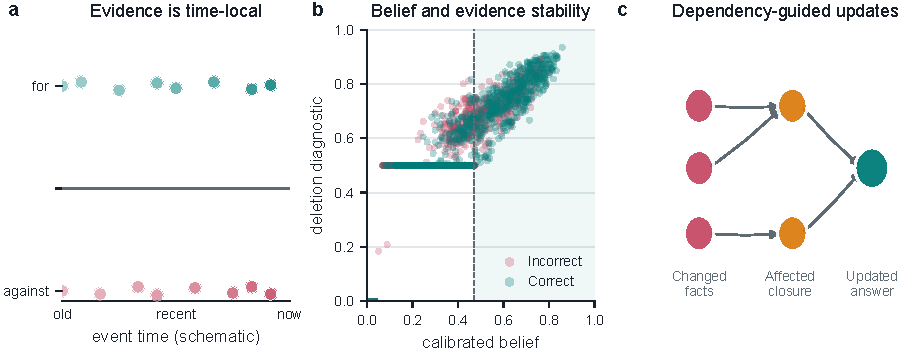
\includegraphics[width=\linewidth]{fig1_concept}
  \caption{\textbf{The StableKG decision layer.} (a) Evidence for a candidate object is time-local and receives a decaying weight. (b) Calibrated belief and the deletion diagnostic describe different aspects of a prediction; all 5,000 ICEWS14 test queries are shown, and the shaded region marks the seed-0 acceptance threshold selected at a 20\% validation target. (c) A changed fact is propagated through the reverse dependency closure, so only affected derived summaries and answers are updated.}
  \label{fig:concept}
\end{figure}

\subsection{Evidence-aware selection lowers accepted risk}
We evaluated published $\mathrm{Pe}$ point queries from three TFLEX-format archives: ICEWS14, ICEWS05-15 and GDELT. Training events form the evidence index, with a cutoff at the query timestamp. Each split contributes 5,000 deterministically spaced validation and test queries. The base scorer's filtered ranking establishes the prediction task (Table~\ref{tab:ranking}); the selective layer changes the order in which predictions are accepted without changing the candidate ranking.

\begin{table}[!htbp]
\centering
\caption{Causal filtered ranking on the public test queries. Ranking is deterministic once the evidence index is fixed.}
\label{tab:ranking}
\small
\resizebox{\linewidth}{!}{%
\begin{tabular}{lrrrrrrr}
\toprule
Dataset & Entities & Train events & Test queries & MRR & Hits@1 & Hits@3 & Hits@10\\
\midrule
ICEWS14 & 7,128 & 72,826 & 5,000 & 0.3153 & 0.2654 & 0.3526 & 0.4012\\
ICEWS05-15 & 10,488 & 368,962 & 5,000 & 0.4221 & 0.3510 & 0.4679 & 0.5536\\
GDELT & 500 & 2,308,165 & 5,000 & 0.2454 & 0.1549 & 0.2715 & 0.4295\\
\bottomrule
\end{tabular}
}
\end{table}

The evidence-aware selector improved the full risk--coverage ordering on both ICEWS benchmarks. On ICEWS14, AURC decreased from 0.5872 to 0.5494; the seed-0 paired timestamp-block difference was -0.0365 (95\% CI -0.0446 to -0.0287). On ICEWS05-15, AURC decreased from 0.5011 to 0.4669; the seed-0 paired timestamp-block difference was -0.0353 (95\% CI -0.0438 to -0.0274). At exactly 20\% test coverage (1,000 accepted queries per method), risk decreased from 0.5060 to 0.4390 and from 0.4070 to 0.3230, respectively; paired timestamp-block intervals for both risk differences excluded zero (Supplementary Table~S8). On GDELT, AURC changed from 0.7694 to 0.7647; the 40\% operating point showed a small risk increase (Supplementary Table~S1). Figure~\ref{fig:risk} shows the complete curves; Supplementary Table~S2 reports paired intervals under frozen validation thresholds.

\begin{figure}[!htbp]
  \centering
  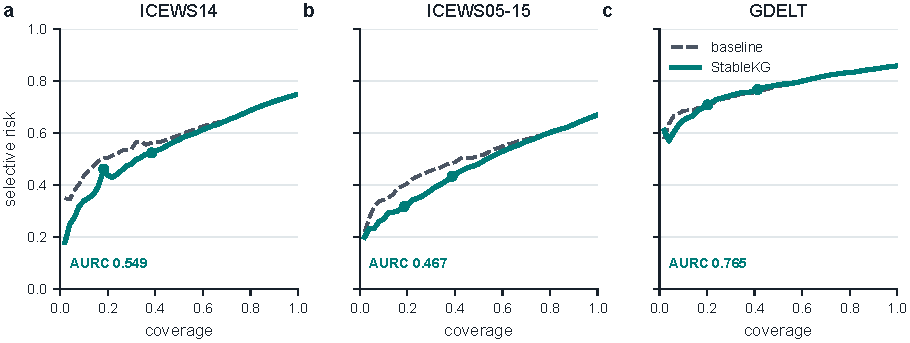
\includegraphics[width=\linewidth]{fig2_risk_coverage}
  \caption{\textbf{Selective risk--coverage curves.} Each panel reports the test risk after sorting predictions by the belief-only baseline or the StableKG belief. Curves, points and AURC use calibration seed 0. Points show the actual test coverage and risk obtained at thresholds selected for 20\% and 40\% validation coverage; Tables S1 and S2 report seed aggregates and uncertainty.}
  \label{fig:risk}
\end{figure}

The same evidence features also improved probability calibration on the ICEWS datasets. On ICEWS14, Brier score changed from 0.1560 to 0.1426 and ten-bin expected calibration error (ECE) from 0.0405 to 0.0158. On ICEWS05-15, Brier score changed from 0.1889 to 0.1720 and ten-bin expected calibration error (ECE) from 0.0410 to 0.0189. Figure~\ref{fig:reliability} displays seed-0 reliability across all test queries; aggregate values for all three datasets are in Supplementary Table~S1.

\begin{figure}[!htbp]
  \centering
  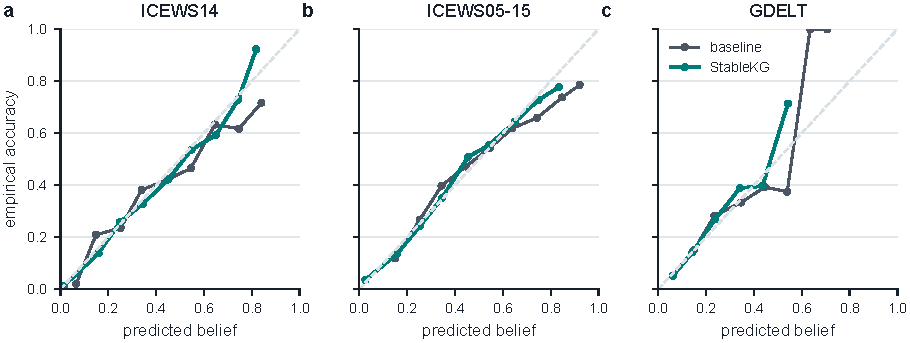
\includegraphics[width=\linewidth]{fig6_reliability}
  \caption{\textbf{Reliability of predicted belief.} Empirical accuracy is plotted against predicted belief in ten bins using all 5,000 test queries and calibration seed 0. The diagonal is perfect calibration. StableKG follows the diagonal more closely on the two ICEWS datasets; the large-scale GDELT panel shows a near-neutral calibration change.}
  \label{fig:reliability}
\end{figure}

\subsection{The decision layer transfers to a learned temporal scorer}
A temporal ComplEx model supplied candidates from learned embeddings, with evidence diagnostics computed for that model's selected object. Across three training seeds, the model achieved MRR 0.3678 on ICEWS14 and 0.4546 on ICEWS05-15. The selective layer reduced AURC from 0.5954 to 0.5570 and from 0.5437 to 0.4701, respectively (Table~\ref{tab:neural}). This transfer shows that evidence features can improve acceptance decisions for learned predictions as well as for the additive scorer. Calibration variation across the two settings is reported alongside selective risk.

\begin{table}[!htbp]
\centering
\caption{Neural-backbone confirmation. Values are means over three training seeds. StableKG is applied after the backbone score and uses the same validation-only operating protocol.}
\label{tab:neural}
\small
\begin{tabular}{lrrrrr}
\toprule
Dataset & MRR & AURC B & AURC S & ECE B & ECE S\\
\midrule
ICEWS14 & 0.3678 & 0.5954 & 0.5570 & 0.0343 & 0.0360\\
ICEWS05-15 & 0.4546 & 0.5437 & 0.4701 & 0.0243 & 0.0227\\
\bottomrule
\end{tabular}
\end{table}

\subsection{Recent temporal backbones retain the evidence-aware gain}
To test transfer to a current high-capacity temporal encoder, we ran the public author implementation of TeRDy (ACL 2025) under the same 5,000-query Pe panel, candidate vocabulary and validation-only selection protocol. On ICEWS14 (rank 6,000; 12 epochs), TeRDy reached MRR 0.6571; StableKG reduced AURC from 0.3801 for the calibrated-score comparator to 0.2896 and exact-20\% risk from 0.1880 to 0.1530. On ICEWS05-15, the author default rank 8,000 exceeded the available 8-GB GPU memory; the pre-specified rank-2,000 adaptation completed 8 epochs and reached MRR 0.5355, with AURC changing from 0.3801 to 0.3716 and exact-20\% risk from 0.2330 to 0.2210. The scoring equations and regularizers are unchanged; rank and resource outcomes are recorded with each checkpoint.

\begin{table}[!htbp]
\centering
\caption{Recent author-code backbone comparison. B is the validation-selected calibrated-score comparator and S is StableKG.}
\label{tab:recent}
\small
\resizebox{\linewidth}{!}{%
\begin{tabular}{lrrrrrr}
\toprule
Dataset & Rank & Epochs & MRR & AURC B & AURC S & Risk20 B/S\\
\midrule
ICEWS14 & 6000 & 12 & 0.6571 & 0.3801 & 0.2896 & 0.1880/0.1530\\
ICEWS05-15 & 2000 & 8 & 0.5355 & 0.3801 & 0.3716 & 0.2330/0.2210\\
\bottomrule
\end{tabular}}
\end{table}

\subsection{Chronological replay preserves the decision advantage}
We then evaluated decisions before revealing the events they predict. The first 70\% of unique timestamps supplied the initial history, the next 15\% supplied validation and the final 15\% supplied test. Every query at a timestamp was scored before any event at that timestamp entered the index. On ICEWS14, AURC changed from 0.4705 to 0.4411 and risk near the 20\% validation target from 0.3665 to 0.2686. On ICEWS05-15, AURC changed from 0.4254 to 0.3957 and risk near the 20\% validation target from 0.3222 to 0.2342. This replay extends the selective advantage to a strict predict-before-reveal setting (Fig.~\ref{fig:temporal}a,b). The corresponding realized coverage remains visible across timestamp blocks (panels c,d), connecting the observed risk to the fraction of decisions accepted.

\begin{figure}[!htbp]
  \centering
  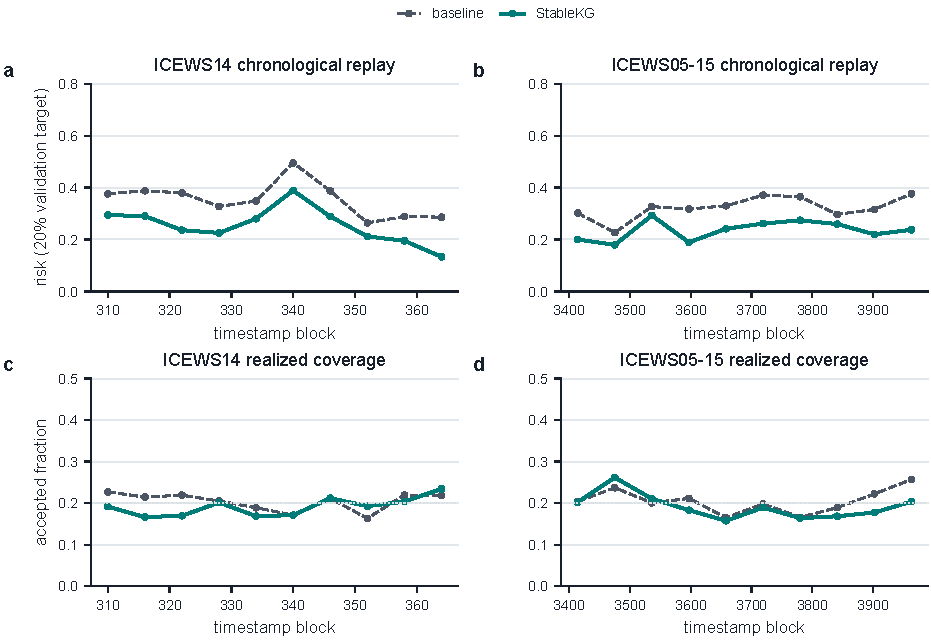
\includegraphics[width=0.98\linewidth]{fig4_temporal}
  \caption{\textbf{Temporal stress tests.} (a,b) Risk under a frozen 20\% validation-target threshold across chronological timestamp blocks for ICEWS14 and ICEWS05-15. (c,d) Realized test coverage in the same blocks for each selector. Horizontal dotted lines mark the 20\% validation target. All four panels use chronological predict-before-reveal outputs; thresholds remain fixed throughout test replay.}
  \label{fig:temporal}
\end{figure}

\subsection{Evidence edits expose local decision stability}
We recorded the winner and evidence diagnostics before editing each supported test query. Three independent edits removed the most recent winner event, removed its strongest seven-unit support window, or injected a current-time event for the runner-up. Low diagnostic scores identified conclusions more likely to change under each edit (Fig.~\ref{fig:interventions}). On ICEWS14, window-deletion flip rates were 0.9980 in the lower score quartile and 0.0011 in the upper quartile. On ICEWS05-15, window-deletion flip rates were 0.9978 in the lower score quartile and 0.0000 in the upper quartile. For window survival, the deletion diagnostic achieved AUROC 0.9977, 0.9982, 0.9997 on ICEWS14, ICEWS05-15 and GDELT, compared with 0.9193, 0.8488, 0.9579 for the raw margin. Thus temporal support structure supplies information specific to whole-window deletion. Under single-event injection, raw margin was the strongest diagnostic, as expected for an additive scorer (Supplementary Table~S7).

\begin{figure}[!htbp]
  \centering
  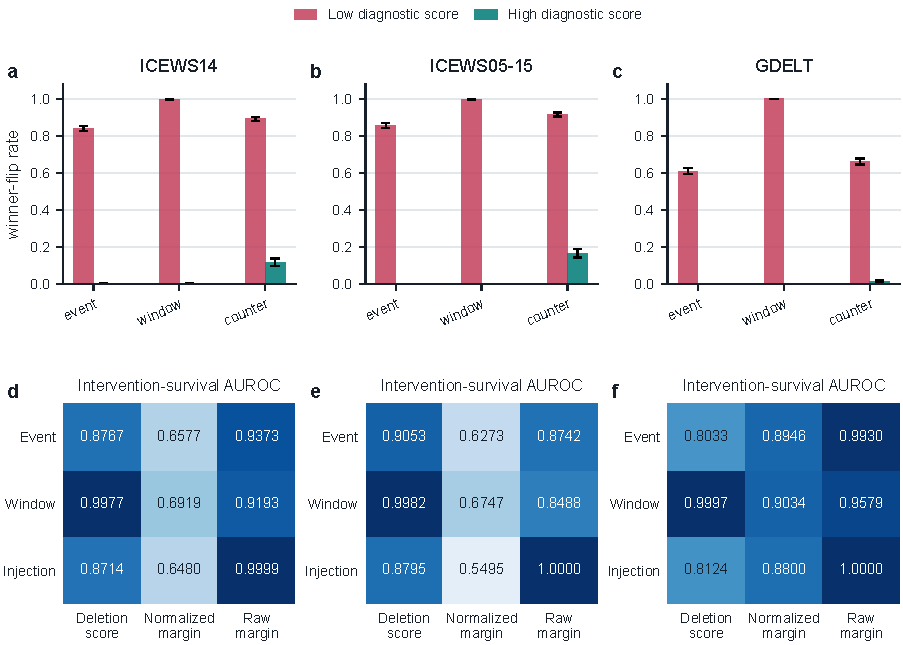
\includegraphics[width=\linewidth]{fig3_interventions}
  \caption{\textbf{Evidence interventions.} Additive-scorer winner-flip rates after a single-event deletion, deletion of the strongest seven-unit winner window, or injection of one current-time counter-event. Bars show the lower and upper certificate quartiles; error bars are bootstrap 95\% intervals over queries. Panels a--c show flip rates for the low/high deletion-diagnostic groups. Panels d--f compare AUROC for predicting survival across the same edits; cells use all supported queries, and darker shading denotes higher AUROC. Deletion score denotes $c$, normalized margin denotes $z$, and raw margin denotes $\Delta$. Query counts are in Supplementary Table~S4.}
  \label{fig:interventions}
\end{figure}

\subsection{Matched controls distinguish selection from diagnosis}
We held margin, support, recency, ridge penalty and validation splits fixed while adding or removing evidence features. Adding the diagnostic score improved ICEWS selection, and adding the normalized margin captured most of the full selector's gain. Together with the intervention controls, this separates two useful roles: normalized evidence separation supports correctness ordering, while temporal support structure identifies susceptibility to window deletion. Table~\ref{tab:matched} reports the matched comparisons; the complete 11-model grid, including softmax/entropy and window-count controls, appears in Supplementary Table~S3.

\begin{table}[t]
\centering
\caption{Matched feature controls. AURC averaged over five validation permutations; lower is better. B contains margin, log-support and recency. $c$ is the deletion diagnostic score, $z$ the normalized margin, and $(f,d)$ the removal cost and diversity.}
\label{tab:matched}
\small
\begin{tabular}{lrrr}
\toprule
Features & ICEWS14 & ICEWS05-15 & GDELT\\
\midrule
Margin only & 0.5681 & 0.4960 & 0.7932\\
B & 0.5872 & 0.5011 & 0.7694\\
B + $c$ & 0.5666 & 0.4818 & 0.7703\\
B + $z$ & 0.5503 & 0.4700 & 0.7657\\
B + $z,f,d$ & 0.5487 & 0.4667 & 0.7648\\
Full ($\mathrm{B}+z,f,d,c$) & 0.5494 & 0.4669 & 0.7647\\
\bottomrule
\end{tabular}
\end{table}

\subsection{Public-graph updates scale with the affected decision set}
We measured the complete event-to-decision maintenance path on all three public archives. The index stores timestamp multiplicities, seven-unit evidence bins, reverse subject--relation lookup and calibrated acceptance outputs for every registered query key. Insertion, deletion and counter-event batches touched 1, 10, 100 or 1,000 events; a clock advance refreshed all decisions. Across 10 repetitions, incremental outputs matched full indexed refresh and an independent raw-event oracle below $10^{-14}$, including winner identity, certificate count and acceptance. For a batch of 100 events, the incremental path refreshed 98.2, 97.7 and 98.7 decisions on average on ICEWS14, ICEWS05-15 and GDELT, compared with 21,667, 51,292 and 9,741 decisions for full refresh. Mean times were 136.3 to 1.3~ms, 363.6 to 2.2~ms and 223.0 to 4.5~ms, respectively (Table~\ref{tab:publicupdates}). A global clock advance correctly refreshes every decision because decay changes all margins; its measured costs were 126, 359 and 228~ms. Resident index growth was 38.1, 144.3 and 515.9~MB, with the largest value corresponding to the 2.3-million-event GDELT archive.

\begin{table}[!htbp]
\centering
\caption{End-to-end public-graph update maintenance. Means over 10 repetitions; full refresh re-evaluates every registered decision from the same indexed summaries.}
\label{tab:publicupdates}
\small
\resizebox{\linewidth}{!}{%
\begin{tabular}{lrrrrrr}
\toprule
Dataset & Events & Decisions & Batch & Full ms & Incremental ms & Refreshed\\
\midrule
ICEWS14 & 72,826 & 21,667 & 100 & 136.3 & 1.3 & 98.2\\
ICEWS05-15 & 368,962 & 51,292 & 100 & 363.6 & 2.2 & 97.7\\
GDELT & 2,308,165 & 9,741 & 100 & 223.0 & 4.5 & 98.7\\
\bottomrule
\end{tabular}}
\end{table}

\subsection{Dependency closure reduces exact recomputation work}
We evaluated incremental maintenance in a separate controlled rule graph with 220 nodes and 20 independent seeds. The affected closure contained 62.6 nodes on average, reducing visited nodes by 71.6\% (95\% CI 70.7--72.3\%). With the closure cached, propagation time decreased from 0.881 to 0.455 ms, a 47.7\% reduction (95\% CI 42.2--52.8\%). Full and incremental outputs agreed exactly for every seed (Fig.~\ref{fig:efficiency}). This experiment verifies the dependency-closure algorithm for deterministic rule propagation; it measures that computation separately from the public TKGC scorer.

\begin{figure}[!htbp]
  \centering
  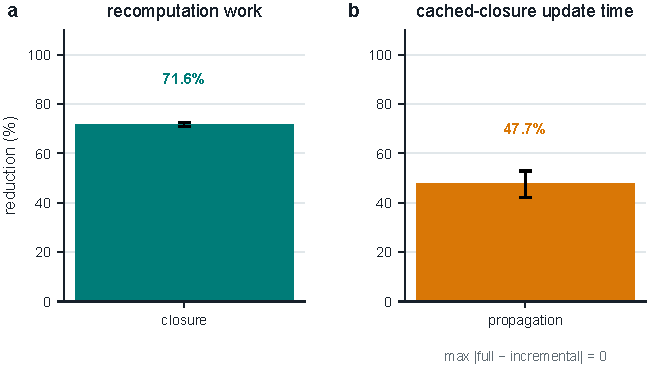
\includegraphics[width=0.78\linewidth]{fig5_efficiency}
  \caption{\textbf{Exact incremental updates.} (a) Fractional reduction in dependency nodes visited by the closure update. (b) Fractional reduction in propagation time with a precomputed closure. Bars show means over 20 controlled seeds and error bars show 95\% bootstrap intervals. Full and incremental recomputation agree exactly in all seeds.}
  \label{fig:efficiency}
\end{figure}

\section{Discussion}
The results connect two decisions that are often evaluated separately: whether a graph prediction is correct enough to accept, and how its evidence can change the answer. \StableKG{} makes this connection inspectable. Calibration orders predictions by empirical correctness, the discrete certificate describes resistance to whole-window deletion under the additive scorer, and continuous diagnostics expose the concentration of support. Their roles are complementary at the protocol level: correctness ordering and sensitivity to evidence edits are different measurable outcomes.

The matched controls sharpen this interpretation. A normalized margin accounts for much of the selective gain, while the deletion diagnostic more accurately identifies susceptibility to window removal than raw margin. The strongest descriptor therefore depends on the decision being made: accepting a prediction and anticipating the effect of an evidence edit call for different summaries. Neural transfer and chronological replay connect this distinction to learned predictions and sequentially revealed histories. Dataset-specific operating behavior is visible in the full risk--coverage results.

Recent work on temporal evidence selection, graph editing and memory-based graph representations provides natural settings for such decision layers \citep{dao2025hgct,fan2026editing,jin2025memorywalk,liu2025terdy}. The TeRDy transfer and public-graph maintenance experiments show that the protocol remains useful as the predictive encoder and event volume change. The additive certificate supplies an exact local guarantee, while the indexed implementation provides an auditable route from event edits to refreshed decisions.

\section{Conclusion}
\StableKG{} connects calibrated acceptance with explicit evidence dependence in temporal knowledge graph reasoning. It improves selective decisions on two public ICEWS benchmarks, transfers to a learned temporal scorer, and retains its advantage during chronological replay. Direct interventions make the relation between support structure and answer stability measurable, while dependency closure provides an exact mechanism for maintaining derived conclusions efficiently. Together, these results establish an inspectable foundation for deciding which evolving graph predictions to use and when to revisit their supporting evidence.

\section{Methods}

\subsection{Task and causal evidence index}
We represent a point query as $q=(s,r,t)$ with a set of labelled objects $A_q$. The training split supplies timestamped observations $(t_i,o_i)$ for each subject--relation pair. The evidence available to $q$ is
\begin{equation}
 E_q=\{(t_i,o_i): (s,r,t_i,o_i)\text{ is in the evidence index and }t_i\leq t\}.
\end{equation}
The inequality is applied before every score, including interventions. Known answers at the same query key are used only for filtered ranking, separately from the scoring evidence. Events are sorted by timestamp and queried with an upper-bound search, so the condition is explicit in the implementation.

For a half-life $h=35$ timestamp units, an observation receives weight
\begin{equation}
 w_i=\exp\left[-\log(2)\frac{t-t_i}{h}\right], \qquad M(o)=\sum_{i:o_i=o}w_i.
\end{equation}
The winner $\hat{o}$ is the object with largest $M(o)$; raw support count and object identifier provide deterministic ties. Let $o_{(2)}$ be the runner-up and $\Delta=M(\hat{o})-M(o_{(2)})$. The public ranker reports filtered average-tie ranks for every labelled answer, averaging reciprocal ranks over all answers rather than selecting the most favourable answer.

\subsection{Window-deletion certificate and continuous diagnostics}
Partition winner evidence into bins $k=\lfloor t_i/7\rfloor$, each spanning seven integer timestamp units. Let $v_1\geq\cdots\geq v_B>0$ be the sorted bin masses, $M=\sum_jv_j$, and $\Delta>0$ the winner margin with competitor evidence fixed. Define
\begin{equation}
 k_*(q)=\min\left\{k:\sum_{j=1}^{k}v_j\geq\Delta\right\},\qquad
 f(q)=\frac{\sum_{j=1}^{k_*}v_j}{M}.
\end{equation}
\textbf{Deletion guarantee.} Every deletion of fewer than $k_*$ whole winner windows leaves a strictly positive margin; some deletion of $k_*$ windows erases that margin. To see this, any subset of $j$ windows has total mass no greater than the $j$ largest masses. All prefixes shorter than $k_*$ sum to less than $\Delta$, and the $k_*$ prefix reaches it. This proves both statements. Equality erases the strict margin but can retain the original answer under deterministic tie-breaking.

The count $k_*$ is the discrete certificate. The associated $f$ records the mass cost of the descending-prefix attack. Zero evidence or a non-positive margin gives $k_*=f=0$. The implementation handles floating-point differences when a full-mass deletion reaches the margin. The continuous descriptors below serve calibration and intervention diagnosis.

Temporal diversity and the continuous deletion diagnostic are
\begin{equation}
 d(q)=1-\frac{v_1}{M},\qquad c(q)=\frac{f(q)+d(q)}{2},
\end{equation}
with $d=0$ when $M=0$. The normalized evidence margin is
\begin{equation}
 z(q)=\operatorname{clip}\left(\frac{\Delta}{M(\hat o)+M(o_{(2)})+10^{-12}},0,1\right).
\end{equation}
An added runner-up mass of $\Delta$ erases the strict margin when other masses are fixed; $z$ expresses that gap relative to the top-two mass. It is a calibration feature, distinct from the fixed one-event injection experiment. For neural candidates, these diagnostics use the selected candidate's evidence and strongest evidence competitor, clipping a negative evidence margin to zero. They describe the evidence scorer associated with that candidate.

\subsection{Calibration and selective decision rule}
The belief-only baseline uses standardized margin, log-support and recency features. The full selector adds certificate, diversity, fragility cost and counter-evidence cost. A ridge logistic model is fitted on the first half of the validation queries after a fixed random permutation:
\begin{equation}
 b(q)=\sigma\left(\beta_0+\beta^{\mathsf T}\operatorname{standardize}(x(q))\right),
\end{equation}
where $\sigma$ is the logistic function and the ridge penalty is $10^{-2}$. The second validation half chooses the threshold closest to each target coverage (20\%, 40\%, 60\% or 80\%); ties retain the higher coverage and then the higher threshold. Test labels are not read during calibration or threshold selection. The selected set is $\mathcal{S}_\tau=\{q:b(q)\geq\tau\}$, its coverage is $|\mathcal{S}_\tau|/|Q|$, and its risk is the mean of $1-\mathbb{1}[\hat{o}\in A_q]$ over $\mathcal{S}_\tau$.

We report Brier score and ten-bin ECE for calibration, AURC for the full risk--coverage ordering, and risk at the operating points. Public results use five seeds for the validation permutation. Neural confirmation uses three training seeds. Paired uncertainty for public risk differences uses 1,000 resamples of contiguous timestamp blocks; seed summaries use 5,000 bootstrap resamples. All intervals are percentile 95\% intervals.

\subsection{Interventions}
For each retained public test query with causal winner evidence, we first record the unedited winner and certificate. Three edits are then evaluated independently: (i) remove the most recent winner event; (ii) remove all winner events in the seven-unit bin with largest weighted mass; and (iii) inject one event at the query timestamp for the runner-up. The edit is scored with the same causal winner rule. A flip is recorded when the edited winner differs from the original. Certificate quartiles are computed per dataset, and flip rates are reported for the lower and upper quartiles. Spearman correlation is computed between certificate and the binary survival outcome. This audit measures the operational semantics of $c(q)$ and does not use the ground-truth answer to select an intervention.

\subsection{Chronological replay and incremental closure}
For chronological replay, all point queries are sorted by timestamp. The earliest 70\% of unique timestamps are used for the initial history, the next 15\% for validation and the latest 15\% for test. At timestamp $t$, all queries are predicted against the current index and only then are events at $t$ appended. The first half of validation timestamps fits the calibrator and the second half sets operating thresholds.

The controlled update graph contains base-fact and derived-rule nodes. Reverse edges connect each premise to rules that read it. For a changed base set, traversal collects all reachable derived nodes; recomputation follows their topological order. Each rule aggregates premise values as one half their minimum plus one half their mean, and a conclusion takes the maximum over its rules. The runtime comparison perturbs 10\% of base nodes and times 2,000 propagation repetitions with the closure precomputed. Closure discovery is outside that timing. Node-count reduction is measured over the dynamic stream's changed-base sets, while runtime uses a separately sampled update set. Full and incremental outputs are compared elementwise.

\subsection{Data and implementation}
We use the ICEWS14, ICEWS05-15 and GDELT TFLEX-format mirrors. We retain the published $\mathrm{Pe}$ point queries and treat each answer list as a set. Archive URLs, mirror revisions, access date, reported license metadata, sizes and SHA-256 hashes are recorded in \texttt{data/DATA\_MANIFEST.md}. The public benchmark evaluates a deterministic evenly spaced cap of 5,000 validation and test queries; the full archive remains available through the documented download command.

The neural confirmation model is a reciprocal temporal ComplEx implementation with complex dimension 96, AdamW optimization, learning rate $2\times10^{-3}$, weight decay $10^{-6}$, 30 epochs and 32 negative samples. ICEWS14 uses batch size 2,048 and ICEWS05-15 uses 4,096. We additionally ran the public TeRDy implementation (ACL 2025) with its published scoring equations and regularizers: rank 6,000 for ICEWS14 (12 epochs) and rank 2,000 for ICEWS05-15 (8 epochs after the rank-8,000 default exceeded 8-GB memory). Checkpoint selection and calibration use disjoint validation subsets. The event-maintenance benchmark records insertion, deletion, counter-event and clock-advance costs on every public archive, including reverse lookup, summary updates and resident memory. All random seeds, thresholds and source-data paths are written to CSV and JSON sidecars. The complete pipeline is executed by \texttt{run\_all.ps1}; recent-backbone and public-update commands are recorded in the repository README.

\section{Data Availability}
The exact public archives used in this study are available from the versioned TFLEX mirrors listed in \texttt{data/DATA\_MANIFEST.md}, together with archive hashes and retrieval metadata. The point-query format is supplied by TFLEX; its source repository and archive landing pages are linked in the manifest. Derived prediction rows, intervention outcomes, aggregate analysis tables and figure source data are included in the repository under \texttt{results\_final\_v5/analysis/} and \texttt{figures/out/}. The mirror metadata reported Apache-2.0 on 7 September 2026; users should consult the source repository terms when redistributing the archives.

\section{Code Availability}
All code needed to download, verify, parse, evaluate, calibrate, intervene, update and plot the reported results is included in this submission package. The fixed entry point is \texttt{run\_all.ps1}; tests are in \texttt{tests/}; dependency bounds and the tested environment are recorded in \texttt{requirements.txt} and \texttt{requirements-lock.txt}. No credentials are required for the public data download.

\section{AI-use disclosure}
OpenAI Codex assisted with research planning, software implementation, execution of experiments, statistical analysis, figure generation, literature metadata checking and manuscript drafting. Experimental values were produced by the accompanying executable code and linked to saved outputs. The author is responsible for reviewing the methods, data provenance, interpretation, references and final manuscript before submission.

\section*{CRediT authorship contribution statement}
Yanbo Bian: Conceptualization, Methodology, Software, Data curation, Formal analysis, Validation, Visualization, Writing -- original draft, Writing -- review and editing.

\section*{Funding}
Funding information to be completed by the author before submission.

\section*{Declaration of competing interest}
The authors declare no competing interests.

\section*{Acknowledgements}
We thank the maintainers of the public ICEWS, GDELT and TFLEX data distributions for making the benchmark archives available.

\fontsize{9}{10.6}\selectfont
\setlength{\bibsep}{0pt}
\bibliographystyle{elsarticle-num}
\bibliography{references}

\end{document}
